\chapter{离子通道} \label{chap:chap8}

大脑中的信号传递取决于神经细胞对极微小刺激做出反应的能力,即细胞膜上的电位差发生快速而巨大的变化。
在感觉细胞中,膜电位的变化是对微小物理刺激的反应:
眼睛中的受体对单个光子作出反应;
嗅觉神经元检测单个气味分子;
内耳中的毛细胞对原子尺寸的微小运动作出反应。
这些感觉反应最终导致动作电位的激发,在此期间膜电位以每秒 500 伏特的速度变化。


作为整个神经系统信号传递的基础,膜电位的快速变化是由膜上称为离子通道的特殊孔隙或开口介导的。
神经细胞的离子通道经过优化和调整,能够对特定的物理和化学信号做出反应。
它们还具有异质性--神经系统的不同部位有不同类型的通道执行特定的信号任务。


由于离子通道在电信号传递中的关键作用,它们的功能失常会导致多种神经系统疾病(第~\ref{chap:chap57}~和~\ref{chap:chap58}~章)。
由离子通道功能失调引起的疾病并不局限于大脑;
例如,囊性纤维化、骨骼肌疾病和某些类型的心律失常也是由离子通道功能失调引起的。
此外,离子通道通常是药物、毒物或毒素的作用部位。
因此,离子通道在神经系统的正常生理学和病理生理学中都具有至关重要的作用。

除了离子通道,神经细胞还含有第二类重要的蛋白质,专门在细胞膜上移动离子,即离子转运蛋白和泵。
这些蛋白质不参与快速神经元信号传导,但对于建立和维持细胞内外具有重要生理意义的离子浓度梯度非常重要。
正如我们将在本章和下一章中看到的,离子转运蛋白和离子泵在一些重要的方面与离子通道不同,但它们也有某些共同特征。


离子通道具有 3 个重要特性:
(1)它们识别和选择特定离子;
(2)它们根据特定的电气、化学或机械信号而打开和关闭;
(3)它们传导离子穿过膜。
神经和肌肉中的通道能以极快的速度将离子传导过细胞膜,从而提供大量电荷流。
单个通道每秒可通过多达 1 亿个离子。
这种电流导致信号传递所需的膜电位快速变化(第~\ref{chap:chap10}~章)。
离子在通道中的流动速度相当于最快的酶--过氧化氢酶和碳酸酐酶--的周转率,后者受到底物扩散的限制。
(大多数其他酶的周转率要慢得多,从每秒 10 到 1 千不等)。


尽管离子流速如此之快,但通道对它们允许渗透的离子具有惊人的选择性。
每种类型的通道仅允许一种或几种类型的离子通过。
例如,神经细胞的负静息电位主要由一类 \ce{K+} 通道决定,这些通道对~\ce{K+} 的渗透性比对~\ce{Na+} 高 100 倍。
相反,动作电位的产生涉及一类~\ce{Na+} 通道,它们对~\ce{Na+} 的渗透性比对~\ce{K+} 的渗透性高 10 到 20 倍。
因此,神经元信号转导的多功能性的关键是不同类别离子通道的调节激活,每个离子通道都对特定离子具有选择性。


许多通道的开启和关闭都是对特定事件的响应:
电压门控通道由膜电位的变化调节,配体门控通道由化学递质的结合调节,机械门控通道由膜拉伸调节。
当细胞静止时,其他通道通常是开放的。
通过这些“静止”通道的离子流在很大程度上决定了静息电位。


离子通过离子通道的流动是被动的,不需要通道消耗代谢能量。
离子通道仅限于催化离子沿着热力学浓度梯度和电梯度被动移动。
这种离子流的方向不是由通道本身决定的,而是由跨膜的静电和扩散驱动力决定的。
例如,\ce{Na+} 离子在动作电位期间通过电压门控~\ce{Na+} 通道流入细胞,因为外部~\ce{Na+} 浓度远大于内部浓度;
开放通道允许~\ce{Na+} 沿着浓度梯度扩散到细胞中。
在这种被动的离子移动过程中,如果没有离子泵,\ce{Na+} 的浓度梯度最终会消失。
不同类型的离子泵可以维持~\ce{Na+}、\ce{K+}、\ce{Ca^2+} 和其他离子的浓度梯度。


这些泵在两个重要细节上不同于离子通道。
首先,开放的离子通道具有一条连续的充满水的通道,离子通过该通道畅通无阻地从膜的一侧流向另一侧,而泵每次移动一个或一组离子穿过膜时,都必须经历一系列构象变化。
因此,通过泵的离子流速度比通过通道慢 100 到 10 万倍。
其次,维持离子梯度的泵使用化学能(通常以\textit{三磷酸腺苷酶}的形式)来逆着电梯度和化学梯度输送离子。
这种离子运动称为主动传输。
离子泵和转运体的功能和结构将在本章末尾和第~\ref{chap:chap9}~章中详细讨论。


在本章中,我们将研究 6 个问题:为什么神经细胞有通道?
通道如何以如此高的速率传导离子并且仍然具有选择性? 
通道是如何门控的?
这些通道的特性如何被各种内在和外在条件所改变?
通道结构如何解释功能?
最后,通过通道的离子运动与通过转运蛋白的离子运动有何不同?
在后续章节中,我们将考虑静息通道和泵如何产生静息电位(第~\ref{chap:chap9}~章)、电压门控通道如何产生动作电位(第~\ref{chap:chap10}~章)以及配体门控通道如何产生突触电位(第~\ref{chap:chap11}、\ref{chap:chap12} 和~\ref{chap:chap13})。



\section{离子通道是跨越细胞膜的蛋白质}

要理解为什么神经细胞使用通道,我们需要了解质膜的性质和溶液中离子的物理化学性质。
所有细胞(包括神经细胞)的质膜厚度约为 6 至 8 纳米,由脂质和蛋白质镶嵌而成。
膜的核心由大约 3 至 4 纳米厚的双层磷脂形成。
在这个连续的脂质薄层中嵌入了包括离子通道在内的整体膜蛋白。


膜的脂质不与水混合,即它们是疏水的。
与之相反的是,如图~\ref{fig:8_1}~所示,细胞内和细胞外的离子会强烈吸引水分子,即它们是亲水性的。
离子吸引水是因为水分子具有双极性:虽然水分子上的净电荷为零,但分子内的电荷是分离的。
水分子中的氧原子倾向于吸引电子,因此带有少量的净负电荷,而氢原子倾向于失去电子,因此带有少量的净正电荷。
由于电荷分布不均,带正电荷的离子(阳离子)会被水的氧原子强烈吸引,而带负电荷的离子(阴离子)则会被氢原子吸引。
同样,如图~\ref{fig:8_1}~所示,离子也会吸引水;
它们会被静电结合的水合水包围。


\begin{figure}[htbp]
	\centering
	\includegraphics[width=0.91\linewidth]{chap08/fig_8_1}
	\caption{细胞膜对离子的渗透性取决于离子与水、膜脂双层和离子通道的相互作用。
		溶液中的离子被一团水分子(水合水)包围,这些水分子被离子的净电荷吸引。
		当离子在溶液中扩散时,该云被离子携带,增加了离子的有效尺寸。
		离子离开这个极性环境进入由磷脂形成的脂质双层的非极性环境在能量上是不利的,因此不太可能。
		磷脂具有亲水性头部和疏水性尾部。
		疏水性尾巴连接在一起以排除水和离子,而极性亲水性头部则面向细胞外液和细胞质的水性环境。
		磷脂由甘油主链组成,其中两个 -OH 基团通过酯键与脂肪酸分子相连。
		甘油的第 3 个-OH基团与磷酸相连。
		磷酸基团进一步连接到各种小的极性醇头基团(R)之一。
		离子通道是跨越脂质双层的完整膜蛋白,为离子穿过膜提供了途径。
		这些通道对特定离子具有选择性。
		钾通道具有排除~\ce{Na+} 的窄孔。
		虽然 \ce{Na+} 离子比 \ce{K+} 离子小,但在溶液中,\ce{Na+} 的有效直径更大,因为它的局部场强更强,导致它吸引更大的水分子云。
		\ce{K+} 通道孔太窄,水合 \ce{Na+} 离子无法渗透。
		钠通道具有选择性过滤器,可弱结合 \ce{Na+} 离子。
		根据\textit{贝蒂尔$\cdot$希勒}及其同事提出的假设,\ce{Na+} 离子在穿过过滤器时会在活性位点短暂结合。
		在结合位点,离子的正电荷被通道壁上带负电荷的氨基酸残基和被通道壁另一侧第二极性氨基酸残基吸引的水分子稳定。
		人们认为,\ce{K+} 离子由于其直径较大,无法通过负电荷有效稳定,因此会被过滤器排除。}
	\label{fig:8_1}
\end{figure}


除非消耗大量能量来克服离子与周围水分子之间的吸引力,否则离子无法从水中进入膜中脂质双分子层不带电的碳氢化合物尾部。
因此,离子从溶液中进入脂质双分子层的可能性极小,所以双分子层本身几乎完全不能渗透离子。
相反,离子会通过离子通道穿过膜,离子通道的能量有利于离子的移动。


虽然人们对离子通道分子性质的确切了解只有大约 35 年的时间,但离子通道的概念可以追溯到 19 世纪末\textit{能斯特$\cdot$布吕克}的研究工作。
生理学家早就知道,尽管细胞膜起着屏障的作用,但细胞膜对水和许多小溶质(包括一些离子)具有渗透性。
为了解释渗透作用,即水在生物膜上的流动,\textit{布吕克}提出,膜上有可以让水流动的通道或孔隙,但不允许较大的溶质流动。
100 多年后,\textit{彼得$\cdot$阿格雷}发现称为水通道蛋白的蛋白质家族形成了对水具有高度选择渗透性的通道。
在 20 世纪初,\textit{威廉$\cdot$贝利斯}提出充满水的通道可以让离子轻松穿过细胞膜,因为离子不需要从水合水中剥离。


离子通过通道移动的想法引出了一个问题:充满水的通道如何能高速传导离子,同时又具有选择性?
例如,通道如何允许 \ce{K+} 离子通过的同时而排除 \ce{Na+} 离子?
选择性不能仅基于离子的直径,因为晶体半径为 0.133 纳米的 \ce{K+} 大于 \ce{Na+}(晶体半径为 0.095 纳米)。
决定离子选择性的一个重要因素是离子水合水壳的大小,因为离子在溶液中移动的难易程度(其迁移率)取决于离子及其周围水壳的大小。
离子越小,其电荷的局部性就越强,电场也就越强。
因此,较小的离子吸引水的能力更强。
因此,当 \ce{Na+} 在溶液中移动时,它对水的更强静电吸引导致它具有一个更大的水壳,这往往会使它的移动速度比 \ce{K+} 慢。
由于其较大的水壳,\ce{Na+} 表现得好像比 \ce{K+} 大。
离子越小,其在溶液中的迁移率越低。
因此,如图~\ref{fig:8_1}~所示,我们可以根据这两种离子在充满水的通道中与水的相互作用,构建一个选择 \ce{K+} 而不是 \ce{Na+} 的通道模型。


尽管此模型解释了通道如何选择 \ce{K+} 并排除 \ce{Na+},但并未解释通道如何选择 \ce{Na+} 并排除 \ce{K+}。
这个问题导致 1930 年代和 40 年代的许多生理学家放弃了通道理论,转而认为离子穿过细胞膜时首先要与特定的载体蛋白结合,然后载体蛋白会使离子穿梭于细胞膜之间。
在这种载体模型中,选择性是基于离子和载体蛋白之间的化学结合,而不是基于离子在溶液中的流动性。


尽管我们现在知道离子可以通过各种转运大分子穿过膜,\textit{钠钾泵}就是一个典型的例子(第~\ref{chap:chap9}~章),但膜离子渗透性的许多特性并不符合载体模型。
最重要的是离子跨膜转移的速度很快。 
当神经递质\textit{乙酰胆碱}与其在神经-肌肉突触的突触后膜中的受体结合时产生的跨膜电流是一个例子。
如后文所述,单个\textit{乙酰胆碱}受体传导的电流为每秒 1250 万个离子。
相比之下,\textit{钠钾泵}每秒最多传输 100 个离子。


如果\textit{乙酰胆碱}受体充当载体,它就必须在 0.1 微秒(百万分之一秒)内将离子转运穿过膜,这是一个令人难以置信的速度。
\textit{钠钾泵}和\textit{乙酰胆碱}受体之间的速率相差 10 万倍,这有力地表明\textit{乙酰胆碱}受体(和其他配体门控受体)必须通过通道传导离子。
后来在许多对 \ce{K+}、\ce{Na+} 和 \ce{Ca^2+} 具有选择性的电压门控通路中进行的测量也证明了单个大分子携带的电流很大,这表明它们也是通道。


但是,我们仍然面临着一个问题:是什么使通道具有选择性?
为了解释选择性,\textit{贝蒂尔$\cdot$希勒}扩展了孔隙理论,提出通道具有像分子筛一样狭窄的区域。
如图~\ref{fig:8_1}~所示,在这个选择性过滤器中,离子必须排出大部分水合水才能穿过通道;
取而代之的是与通道壁上的极性(带电)氨基酸残基形成的弱化学键(静电相互作用)。
由于脱去水合作用水在能量上是不利的,因此只有当离子与选择性过滤器的相互作用能量补偿了离子与其水合作用水的相互作用能量损失时,离子才会穿越通道。
穿过通道的离子通常仅在短时间内(小于 1 微秒)与选择性过滤器结合,之后静电和扩散力推动离子穿过通道。
在孔径大到足以容纳几个水分子的通道中,离子不需要完全脱离其水壳层。


这种化学识别性和特异性是如何建立起来的呢?
\textit{乔治$\cdot$艾森曼}在 1960 年代早期提出了一种理论来解释离子选择性玻璃电极的特性。
根据这一理论,具有高负电场强度的结合位点--例如由谷氨酸或天冬氨酸的带负电的羧酸基团形成的结合位点--将比 \ce{K+} 更紧密地结合 \ce{Na+}。
产生这种选择性的原因是,根据库仑定律,两个带电基团之间的静电相互作用与两个基团之间的距离成反比。


由于 \ce{Na+} 的晶体半径比 \ce{K+} 小,因此它能比 \ce{K+} 更接近具有高负场强的结合位点,从而在结合时获得更有利的自由能变化。
这就弥补了 \ce{Na+} 为了穿过狭窄的选择性过滤器而需要失去部分水合水的不足。
相比之下,负场强较低的结合位点(例如,由极性羰基或羟基氧原子组成的结合位点)会选择~\ce{K+} 而不是 \ce{Na+}。
在这样的位置,\ce{Na+} 的结合不会提供足够的自由能变化来补偿离子的水合水的损失,而 \ce{Na+} 具有很强的水合水。
然而,由于较大的 \ce{K+} 离子与水的相互作用较弱,因此这样的位点将能够补偿 \ce{K+} 离子水合水的损失。
目前认为,离子通道之所以具有选择性,既是因为这种特定的化学作用,也是因为基于孔径的分子筛分作用。



\section{所有细胞中的离子通道都有几个功能特征}

大多数细胞都能够发出局部信号,但只有神经和肌肉细胞专门用于长距离快速信号传递。
虽然神经细胞和肌肉细胞的膜离子通道种类特别丰富,密度也很高,但它们的通道与体内其他细胞的通道并无本质区别。
在这里,我们描述了各种细胞中离子通道的一般特性,这些细胞是通过在各种实验条件下记录流过通道的电流来确定的。



\subsection{可以记录通过单个离子通道的电流}

离子通道的研究最初仅限于记录通过一类离子通道的整个群体的总电流,这种方法掩盖了通道功能的一些细节。
后来的发展使得通过单个离子通道记录电流获得更高的分辨率成为可能。
\textit{厄温$\cdot$内尔}和\textit{伯特$\cdot$萨克曼}于 1976 年首次直接记录了生物膜中的单个离子通道。
他们将含有\textit{乙酰胆碱}(激活骨骼肌膜中\textit{乙酰胆碱}受体的神经递质)的玻璃微量移液器紧紧压在肌肉膜上。
从移液器尖端下方的膜记录代表单个\textit{乙酰胆碱}受体通道打开和关闭的小单一电流脉冲。
当前脉冲都具有相同的幅度,表明通道以全开或全关的方式打开(文本框~\ref{box:8_1})。


\begin{proposition}[单离子通道中的电流记录:膜片钳] \label{box:8_1}
	
	\quad \quad 膜片钳技术是由\textit{厄温$\cdot$内尔}和\textit{伯特$\cdot$萨克曼}于1976年开发的,用于记录单离子通道的电流。
	它是对原始电压箝位技术的改进(见文本框~\ref{box:10_1})。
	
	\quad \quad 将一个尖端直径约为1 微米的小型火抛光玻璃微量移液管压在骨骼肌纤维膜上。
	如图~\ref{fig:8_2}A~所示,与微量移液管中电解质接触的金属电极将移液管连接到一个特殊的回路上,该回路测量通过移液管尖端下膜通道的电流。
	
	\quad \quad 1980年,\textit{内尔}发现,对贴片移液管进行少量抽吸可以大大提高移液管和膜之间的密封性。
	结果是在移液管的内部和外部之间具有极高阻力的密封。
	该密封降低了电子噪声,并将膜片钳技术的实用性扩展到整个离子通道范围。
	如图~\ref{fig:8_2}B~所示,自这一发现以来,膜片钳技术已被用于研究各种神经元和其他细胞中的所有主要类型的离子通道。
	
	\quad \quad \textit{克里斯托弗$\cdot$米勒}独立开发了一种将离子通道从生物膜整合到人工脂质双层中的方法。
	他首先在搅拌器中将膜均质化;
	然后,通过离心匀浆,他分离出仅由膜囊泡组成的部分。
	他使用\textit{保罗$\cdot$穆勒}和\textit{唐纳德$\cdot$鲁丁}在20世纪60年代开发的技术研究了这些囊泡的功能成分。
	他们发现了如何通过在分离两种盐溶液的非导电屏障上的孔上画一薄层磷脂来创建人工脂质双层。
	米勒发现,在适当的离子条件下,他的膜囊泡与平面磷脂膜融合,将囊泡中的任何离子通道结合到平面膜中。
	
	\quad \quad 这种技术有两个实验优势。
	首先,它允许从膜片钳无法接近的细胞区域的离子通道进行记录;
	例如,米勒成功地研究了从骨骼肌内膜(肌浆网)分离的~\ce{K+}~通道。
	其次,它使研究人员能够研究膜脂质的组成如何影响通道功能。
	
\end{proposition}


\begin{figure}[htbp]
	\centering
	\includegraphics[width=0.9\linewidth]{chap08/fig_8_2}
	\caption{膜片钳设置和记录。
	A. 在盐水溶液中含有低浓度\textit{乙酰胆碱}的移液管用于记录通过骨骼肌\textit{乙酰胆碱}受体通道的电流\cite{alberts2017molecular}。
	B. 当通道在\textit{闭合}状态和\textit{打开}状态之间切换时,膜片钳记录通过单个\textit{乙酰胆碱}受体通道的电流。}
	\label{fig:8_2}
\end{figure}



在 -80 毫伏的膜电位下测得的脉冲为 2 皮安(2 × 10$^{-12}$ A),根据欧姆定律(I = V/R)表明通道的电阻为 5 × 10$^{11}$欧姆。
在处理离子通道时,谈论电导更有用,即电阻的倒数($\gamma = 1/R$),因为它提供了与离子渗透性相关的电测量。
因此,单个离子通道的欧姆定律可表示为$i=\gamma \times V$。
\textit{乙酰胆碱}受体通道的电导约为 25 × 10$^{-12}$ 西门子,或 25 皮西门子,其中 1 西门子等于 1 欧姆的倒数。



\subsection{通过通道的离子通量不同于自由溶液中的扩散}

离子渗透的动力学特性最好用通道的电导来描述,通道的电导是通过测量开放通道在电化学驱动力作用下的电流(离子通量)来确定的。
净电化学驱动力由两个因素决定:
跨膜的电势差和跨膜的渗透离子的浓度梯度。
改变其中任何一个因素都可以改变净驱动力(第~\ref{chap:chap9}~章)。


在某些开放通道中,电流随驱动力呈现线性变化:也就是说,通道表现为简单的电阻器。
在其他通道中,电流随驱动力呈非线性变化。
% 整流器:交流电->直流电;反过来为“逆变器”
% 使交变电流形成单向电流
如图~\ref{fig:8_3}~所示,这种类型的通道起到整流器的作用:
由于通道结构或离子环境的不对称性,它在一个方向上比在另一个方向上更容易传导离子。


\begin{figure}[htbp]
	\centering
	\includegraphics[width=0.95\linewidth]{chap08/fig_8_3}
	\caption{电流-电压关系。
		在许多离子通道中,通过开放通道的电流($i$)与膜电压($V_m$)之间的关系是线性的(左图)。
		此类通道被称为“欧姆”通道,因为它们遵循欧姆定律,$i = V_m /R$ 或 $ V_m \times \gamma $,其中 $\gamma$ 是电导。
		在其他通道中,电流和膜电位之间的关系是非线性的。
		这种通道被称为“整流”,因为它比另一个方向更容易在一个方向上传导电流。
		右图显示了一个外向整流通道,对于给定的电压绝对值,正电流(右侧)大于负电流(左侧)。}
	\label{fig:8_3}
\end{figure}


\begin{figure}[htbp]
	\centering
	\includegraphics[width=0.55\linewidth]{chap08/fig_8_4}
	\caption{离子通道打开和关闭的 3 个物理模型。
		A. 通道的一个区域发生局部构象变化。
		B. 沿着河道的长度会发生广义的结构变化。
		C. 阻塞粒子摆动进出通道口。}
	\label{fig:8_4}
\end{figure}


\begin{figure}[htbp]
	\centering
	\includegraphics[width=0.95\linewidth]{chap08/fig_8_5}
	\caption{几种类型的刺激控制离子通道的打开和关闭。
		A. 当配体结合通道蛋白外表面上的受体位点时,配体门控通道打开。配体结合产生的能量将通道推向开放状态。
		B. 一些通道受蛋白质磷酸化和去磷酸化的调节。
		通道开放的能量来自高能磷酸盐$P_i$的转移。
		C. 电压门控通道随着膜上电位差的变化而打开和关闭。
		膜电位的变化通过作用于具有净电荷的通道区域而引起局部构象变化。
		D. 一些通道响应膜拉伸或压力而打开和关闭。
		门控的能量可能来自机械力,这些机械力直接通过膜脂质双层的扭曲或通过附着在细胞骨架或周围组织上的蛋白质丝传递到通道。}
	\label{fig:8_5}
\end{figure}


\begin{figure}[htbp]
	\centering
	\includegraphics[width=0.8\linewidth]{chap08/fig_8_6}
	\caption{电压门控通道通过两种机制失活。
		A. 许多电压门控通道在响应膜的去极化而短暂打开后进入难治(失活)状态。
		只有在膜电位恢复到其静息值后,它们才能从难治状态恢复到静息状态。
		B. 当通道打开后内部\ce{Ca^2+}水平增加时,一些电压依赖性\ce{Ca^2+}通道变得失活。
		内部\ce{Ca^2+}与\textit{钙调蛋白}结合,\textit{钙调蛋白}是与通道相关的特定调节蛋白。}
	\label{fig:8_6}
\end{figure}


\begin{figure}[htbp]
	\centering
	\includegraphics[width=0.8\linewidth]{chap08/fig_8_7}
	\caption{外源配体(例如药物)可以使离子通道偏向开放或闭合状态。
		A. 在通常通过内源性配体(1)的结合打开的通道中,药物或毒素可以通过可逆(2)或不可逆(3)反应阻断激动剂的结合。
		B. 一些外源性药物可以通过与调节位点结合而使通道偏向开放状态,这与通常打开通道的配体结合位点不同。}
	\label{fig:8_7}
\end{figure}


通过通道的净离子通量(电流)的速率取决于周围溶液中渗透离子的浓度。
在低浓度下,电流几乎随浓度线性增加。
在较高浓度下,电流往往会达到一个点,不再增加。
此时,电流被称为饱和。
这种饱和效应表明,细胞膜上的离子通量与自由溶液中的电化学扩散不同,而是涉及离子与通道孔内特定极性位点的结合。
根据简单的电扩散模型预测,离子电流的增加应与浓度的增加成正比。


对于多种离子通道,电流与离子浓度之间的关系可以用一个简单的化学结合方程来很好地描述,该方程与酶的\textit{米氏方程}相同,表明在渗透过程中通道内结合了一个离子。
电流达到其最大值一半时的离子浓度定义了解离常数,即一半通道将被结合离子占据的浓度。
电流与浓度曲线图中的解离常数通常非常高,约为 100 毫摩尔,表明结合较弱(在酶和底物之间的典型相互作用中,解离常数低于 1 微摩尔)。
快速的离子解离是通道实现非常高的传导速率的必要条件,而这种传导速率正是信号传导过程中膜电位快速变化的原因。


某些离子通道会被细胞质或细胞外液中的某些游离离子或分子阻断,这些游离离子或分子会与水孔的孔口或孔内的某处结合。
如果阻断剂是一种与孔内某个部位结合的离子,那么它在进入通道时会受到膜电场的影响。
例如,如果带正电荷的阻断剂从膜外进入通道,那么使膜的细胞质侧更负,就会通过静电吸引将阻断剂驱入通道,从而增加阻滞效果。
虽然有些阻断剂是源自体外的毒素或药物,但有些阻断剂则是细胞或其环境中通常存在的普通离子。
某些类别通道的生理阻断剂包括 \ce{Mg^2+}、\ce{Ca^2+}、\ce{Na+} 和多胺(如精胺)。



\section{离子通道的结构是从生物物理学、生物化学和分子生物学研究中推断出来的}

离子通道是什么样子的?
通道蛋白如何跨膜?
打开和关闭时通道的结构会发生什么变化?
沿着通道蛋白的长度,药物和递质结合在哪里?


生物物理、生物化学和分子生物学研究使人们对通道结构和功能有了基本的了解。
最近利用 X 射线晶体学和低温电子显微镜进行的研究提供了有关越来越多通道原子级结构的信息。
所有离子通道都是大型整合膜蛋白,具有核心跨膜结构域,其中包含跨越整个膜宽度的中央水孔。
通道蛋白通常含有附着在其外表面的碳水化合物基团。 许多通道的成孔区由两个或多个亚基组成,这些亚基可能相同,也可能不同。
此外,一些通道还具有辅助亚基,这些辅助亚基可能具有多种作用,包括促进通道的细胞表面表达、将通道定位到细胞表面的适当位置以及改变通道的门控特性。
如图~\ref{fig:8_8}~所示,这些亚基可能附着在细胞质末端或嵌入细胞膜中。


\begin{figure}[htbp]
	\centering
	\includegraphics[width=1.0\linewidth]{chap08/fig_8_8}
	\caption{离子通道是由多个亚基组成的完整膜蛋白。
		A. 离子通道可以构建为来自不同亚基的异源寡聚体(左),作为来自单一类型亚基的同源寡聚体(中间),或者来自组织成重复基序的单个多肽链,其中每个基序的功能相当于一个亚基(右)。
		B. 除了形成中心孔的一个或多个 $\alpha$ 亚基外,一些通道还包含调节孔门控、通道表达和膜定位的辅助亚基($\beta$ 或 $\gamma$)。}
	\label{fig:8_8}
\end{figure}


% The genes for
所有主要离子通道类别的基因都已被克隆和测序。
从通道的\textit{脱氧核糖核酸}序列推断出的通道氨基酸序列可用于创建通道蛋白的结构模型。
然后,根据使用电子和X射线衍射分析实验确定的相关蛋白质的结构,预测二级结构区域(氨基酸残基排列成$\alpha$-螺旋和$\beta$-片),以及可能对应于通道跨膜结构域的区域。
例如,这类分析发现,在\textit{乙酰胆碱}受体通道亚基的氨基酸序列中存在 4 个疏水区域,每个区域的长度约为 20 个氨基酸。
如图~\ref{fig:8_9}~所示,这些区域中的每一个都被认为形成了一个跨膜的 $\alpha$ 螺旋。


\begin{figure}[htbp]
	\centering
	\includegraphics[width=0.8\linewidth]{chap08/fig_8_9}
	\caption{跨膜蛋白的二级结构。
		A. 骨骼肌中存在的烟碱\textit{乙酰胆碱}受体通道亚基的二级结构。
		每个圆柱体(M1–M4)代表一个假定的跨膜 $\alpha$-螺旋,由大约 20 个疏水氨基酸残基组成。
		膜片段由亲水性残基的细胞质或细胞外片段(环)连接。
		蛋白质的氨基末端(NH2)和羧基末端(COOH)位于膜的细胞外侧。
		B. 离子通道蛋白的跨膜区域可以使用疏水性图来识别。
		从克隆的受体亚基基因的核苷酸序列推断出烟碱型乙酰胆碱受体$\alpha$-亚基的氨基酸序列。
		然后绘制亚基整个氨基酸序列的疏水性移动平均值。
		图中的每个点代表 19 个氨基酸序列的平均疏水指数,对应于序列的中点。
		4 个疏水区域(M1–M4)对应于跨膜片段。
		图中最左边的疏水区域是信号序列,在蛋白质合成过程中,它将蛋白质的亲水氨基末端定位在细胞的细胞外表面。
		信号序列从成熟蛋白上切下\cite{schofield1987sequence}。}
	\label{fig:8_9}
\end{figure}


比较来自不同物种的相同类型通道的氨基酸序列,可以进一步了解通道的结构和功能。
显示高度序列相似性(即在整个进化过程中高度保守)的区域可能对确定通道的结构和功能很重要。
同样,不同但相关类型的通道中的保守区域可能具有共同的生物物理功能。


可以通过多种技术探索通道初级氨基酸序列变化的功能后果。
一种特别通用的方法是使用基因工程构建通道,通道的部分来自不同物种的基因,即所谓的嵌合通道。
该技术利用了相同类型的通道在不同物种中可能具有稍微不同的特性这一事实。
例如,牛的\textit{乙酰胆碱}受体通道的单通道电导略大于电鱼中的\textit{乙酰胆碱}受体通道。
通过将嵌合通道的特性与两个原始通道的特性进行比较,可以评估通道特定区域的功能。
该技术已被用于鉴定形成\textit{乙酰胆碱}受体通道孔内壁的跨膜片段(第~\ref{chap:chap12}~章)。


不同氨基酸残基或残基片段的作用可以通过定点突变进行测试,定点突变是一种基因工程,在这种工程中,特定的氨基酸残基会被替换或删除。
最后,人们可以利用通道基因中自然发生的突变。
神经或肌肉中编码离子通道的基因中存在许多遗传和自发突变,这些突变会导致通道功能发生变化,从而引发某些神经系统疾病。
其中许多突变是由通道蛋白中单个氨基酸的局部变化引起的,这表明该区域对通道功能的重要性。
这些通道的详细功能变化可以在人工表达系统中进行检验。



\subsection{离子通道可以按基因家族进行分组}

人类基因组说明了多细胞生物体中离子通道的多样性。 我们的基因组包含 9 个编码电压门控 \ce{Na+} 通道变体的基因、10 个不同 \ce{Ca^2+} 通道的基因、80 个 \ce{K+} 通道的基因、70 个配体门控通道的基因以及十几个 \ce{Cl-} 通道的基因。
幸运的是,编码离子通道的基因之间的进化关系提供了一个相对简单的框架来对它们进行分类。


大多数在神经和肌肉细胞中描述的离子通道都属于几个基因超家族。
每个基因超家族的成员都有相似的氨基酸序列和跨膜拓扑结构,更重要的是,它们还具有相关的功能。
每个超家族都被认为是由一个共同的祖先基因通过基因复制和分化进化而来。
一些超家族还可进一步细分为编码结构和功能更接近的通道的基因家族。


一个超家族编码配体门控离子通道,这些通道是神经递质\textit{乙酰胆碱}、\textit{$\gamma$-氨基丁酸}、甘氨酸或\textit{5-羟色氨}的受体(第~\ref{chap:chap12}~章)。 
如图~\ref{fig:8_10}A~所示,所有这些受体都由 5 个亚基组成,每个亚基都有 4 个跨膜 $\alpha$ 螺旋。
此外,形成配体受体的 N 末端细胞外结构域包含一个由 13 个氨基酸组成的保守环,两侧是一对形成二硫键的半胱氨酸残基。
因此,该受体超家族被称为\textit{半胱氨酸-环受体}。
除了激动剂之外,配体门控通道还可以根据离子选择性进行分类。
编码谷氨酸受体通道的基因属于一个独立的基因家族。


\begin{figure}[htbp]
	\centering
	\includegraphics[width=0.75\linewidth]{chap08/fig_8_10}
	\caption{离子通道的 3 个超家族。
		A. 配体门控通道大家族的成员,例如\textit{乙酰胆碱}受体通道,由 5 个相同或密切相关的亚基组成,每个亚基包含 4 个跨膜 $\alpha$-螺旋(M1–M4)。
		图中的每个圆柱体代表一个跨膜 $\alpha$-螺旋。
		B. \textit{间隙连接通道}由一对半通道形成,突触前和突触后细胞膜各有一个,连接在两个细胞之间的空间中。
		每个半通道由 6 个相同的亚基组成,每个亚基包含 4 个跨膜 $\alpha$-螺旋。
		间隙连接通道充当电突触中突触前和突触后细胞的细胞质之间的管道(第~\ref{chap:chap11}~章)。
		C. 电压门控~\ce{Na+}~通道由一条多肽链形成,该多肽链包含 4 个同源结构域或重复序列(基序 I-IV),每个具有 6 个跨膜 $\alpha$-螺旋(S1-S6)。
		S5 和 S6 区段由一条延伸的氨基酸链连接,即 P 区,它浸入和浸出膜的外表面,形成孔的选择性过滤器。
		电压门控 \ce{Ca^2+} 通道具有相同的一般结构模式,尽管氨基序列不同。}
	\label{fig:8_10}
\end{figure}




\textit{间隙连接通道}在电突触处连接两个细胞的\textit{细胞质}(第~\ref{chap:chap11}~章),由一个单独的基因超家族编码。
\textit{间隙连接通道}由两个半通道组成,每个半通道来自每个连接的细胞。
如图~\ref{fig:8_10}B~所示,一个半通道有 6 个相同的\textit{亚基},每个亚基有 4 个跨膜片段。


负责产生动作电位的电压门控离子通道的编码基因属于另一个超家族(第~\ref{chap:chap10}~章)。
这些通道对\ce{Ca^2+}、\ce{Na+} 或 \ce{K+} 具有选择性。
\textit{脱氧核糖核酸}序列的比较数据表明,大多数对电压敏感的阳离子通道源于一个共同的祖先通道(可能是 \ce{K+} 通道),可以追溯到 14 亿多年前的单细胞生物,当时植物界和动物界尚未进化分化。


所有电压门控阳离子通道都具有类似的四重对称结构,其核心基序由 6 个跨膜 $\alpha$ 螺旋区段组成,称为 S1–S6。
如图~\ref{fig:8_10}C~和图~\ref{fig:8_11}A~所示,第 7 个疏水区,P 区,通过浸入和浸出膜的细胞外侧连接 S5 和 S6 区段;
它构成了通道的选择性过滤器。
如图~\ref{fig:8_10}C~所示,电压门控 \ce{Na+} 和\ce{Ca^2+}通道由一个大亚基组成,其中包含该基本基序的 4 个重复。
如图~\ref{fig:8_11}A~所示,电压门控 \ce{K+} 通道是四聚体,每个单独的亚基包含一个基本基序的副本。
每个亚基向完全组装通道的孔提供一个 P 区。
这种结构配置与后面和第~\ref{chap:chap10}~章中描述的其他关系更远的通道家族相同。


\begin{figure}[htbp]
	\centering
	\includegraphics[width=0.75\linewidth]{chap08/fig_8_11}
	\caption{具有 P 区的 4 个相关离子通道家族。
		A. 如图~\ref{fig:8_10}C~所示,电压门控 \ce{K+} 通道由 4 个亚基组成,每个亚基对应一个电压门控 \ce{Na+} 或\ce{Ca^2+}通道的重复结构域,具有 6 个跨膜区段和一个成孔 P 区。
		B. 内向整流 \ce{K+} 通道由 4 个亚基组成,每个亚基只有两个由 P 区连接的跨膜区段。
		C. \textit{双孔钾离子通道}由包含两个重复的亚基组成,类似于内向整流 \ce{K+} 通道亚基,每个重复包含一个 P 区。
		这些亚基中的两个结合形成具有 4 个 P 区的通道。
		D. 谷氨酸受体构成了一个独特的具有 P 区的四聚体通道家族。
		它们的孔隙区域对阳离子是非选择性渗透的。
		在这些受体中,氨基末端在细胞外,P 区进出细胞膜的细胞质侧。
		远缘细菌 GluR0 \ce{K+} 可渗透谷氨酸受体有 4 个亚基,其中包含两个跨膜片段(左);
		在高等生物中,亚基包含 3 个(右)。}
	\label{fig:8_11}
\end{figure}


S4 段被认为在电压门控中起着特别重要的作用。
它含有一种特殊的氨基酸模式,其中每隔 3 个位置就含有一个带正电荷的精氨酸或赖氨酸残基。
这一区域最初被认为是电压传感器,因为根据基本的生物物理原理,电压门控必须涉及膜内门控电荷在膜电场中的移动。
人们发现这种正电荷模式在所有电压门控阳离子选择性通道中高度保守,但在非电压门控通道中却不存在,这为 S4 成为电压传感器提供了更多证据。
进一步的证据来自定点诱变实验,该实验表明中和 S4 中的这些正电荷会降低通道激活的电压敏感性。


编码电压门控 \ce{K+} 通道的主要基因家族与另外 3 个 \ce{K+} 通道家族相关,每个家族都具有独特的特性和结构。
其中一个家族包括编码 3 种通道的基因,这些通道由细胞内 \ce{Na+} 或\ce{Ca^2+}或细胞内\ce{Ca^2+}加去极化激活。
第二个家族由编码内向整流 \ce{K+} 通道的基因组成。
由于它们在静息电位下是开放的,并且在去极化过程中迅速被胞质阳离子封闭,因此它们更容易向内而不是向外传导离子。
每个通道亚基只有两个跨膜片段,由一个成孔 P 区连接。
如图~\ref{fig:8_11}~所示,第三个基因家族编码\textit{双孔钾离子通道},该通道由具有两个重复成孔区段的亚基组成。
各种成员受温度、机械力和细胞内配体的调节。
这些通道也可能有助于静息膜的 \ce{K+} 渗透性。


对从细菌到人类的各种物种的基因组进行测序后,人们发现了更多的离子通道基因家族。
其中包括具有相关 P 区的通道,但它们与电压门控通道家族的关系非常疏远。
如图~\ref{fig:8_11}D~所示,一个例子是兴奋性突触后谷氨酸门控通道,其中 P 区倒转,进入和离开膜的内表面。


最后,非选择性阳离子通道的\textit{瞬时受体电位}家族(以突变果蝇菌株命名,其中光在光感受器中引起短暂的受体电位)包含一个非常大且多样化的四聚体通道组,其中包含 P 区。
与电压门控 \ce{K+} 通道一样,\textit{瞬时受体电位}通道也包含 6 个跨膜片段,但在大多数情况下由细胞内或膜内配体门控。
\textit{瞬时受体电位}通道对于所有细胞中的\ce{Ca^2+}代谢、昆虫中的视觉信号以及高等动物神经系统中的痛、热和冷感觉都很重要(第~\ref{chap:chap18}~章)。
\textit{瞬时受体电位}通道与哺乳动物的渗透压感受和某些味觉有关。


人们还发现了许多其他通道家族,它们在结构上与前面提到的那些通道无关。
这些包括有助于设定骨骼肌细胞和某些神经元静息电位的 CLC \ce{Cl-} 通道、由机械刺激激活的非特异性阳离子可渗透压电通道(第~\ref{chap:chap18}~章)、由炎症期间释放的 \ce{H+} 激活的 \ce{Na+} 通道,以及由\textit{三磷酸腺苷酶}激活的配体门控阳离子通道,\textit{三磷酸腺苷酶}在某些兴奋性突触中起神经递质的作用。
随着人类基因组计划的完成,现在几乎所有主要类别的离子通道基因可能都已经被确定了。


离子通道的多样性甚至大于离子通道基因的数量。
由于亚家族中的大多数通道由多个亚基组成,其中每种类型都可能由一个密切相关的基因家族编码,因此这些亚基的组合排列可以产生具有不同功能特性的多种异源多聚体通道。
转录后和翻译后修饰还可产生更多的多样性。
这些结构和功能上的微妙变化可能会使通道发挥高度特异性的功能。
与酶同种型一样,具有略微不同特性的通道变体可能在不同的发育阶段、整个大脑的不同细胞类型甚至细胞内的不同区域中表达。
神经元活动的变化也会导致离子通道表达模式的变化(第~\ref{chap:chap10}~章)。


生物化学、生物物理学和分子生物学方法在定义大量离子通道之间的结构-功能关系方面发挥着重要作用。
利用 X 射线晶体学和低温电子显微镜以原子分辨率确定通道结构,为进一步了解离子通道功能和致病突变导致功能失常的机制提供了一个框架。
将来自这些不同方法的大量数据结合起来,就有可能构建详细的分子模型,这些模型可以通过进一步的实验以及分子动力学模拟等理论方法进行检验。





\subsection{钾通道结构的 X 射线晶体学分析提供了对通道渗透性和选择性机制的深入了解}

\textit{罗德$\cdot$麦金农}及其同事首次对离子选择性通道孔隙区域的分子结构进行了高分辨率 X 射线晶体学分析。
为了克服获取大型整体膜蛋白晶体所固有的困难,他们最初关注的是一种细菌的非电压门控 \ce{K+} 通道,称为 KcsA
如图~\ref{fig:8_11}B~所示,这种通道有利于晶体学的研究,因为它可以高水平表达以进行纯化,体积相对较小,并且具有简单的跨膜拓扑结构,与包括哺乳动物在内的高等生物中的内向整流 \ce{K+}通道类似。


KcsA 蛋白的晶体结构为了解通道促进 \ce{K+} 离子穿过疏水脂质双层移动的机制提供了一些重要信息。
如图~\ref{fig:8_12}A~所示,该通道由围绕中心孔对称排列的 4 个相同亚基组成。
每个亚基都有两个跨膜 $\alpha$ 螺旋,一个内螺旋和一个外螺旋。
它们通过 P 回路连接,形成通道的选择性滤波器。
这些亚基的氨基酸序列与脊椎动物电压门控 \ce{K+} 通道的 S5-P-S6 区域的氨基酸序列同源。
如图~\ref{fig:8_12}B,C~所示,每个亚基的两个 $\alpha$-螺旋从孔的中心轴倾斜,使得结构类似于倒置的圆锥形帐篷。


\begin{figure}[htbp]
	\centering
	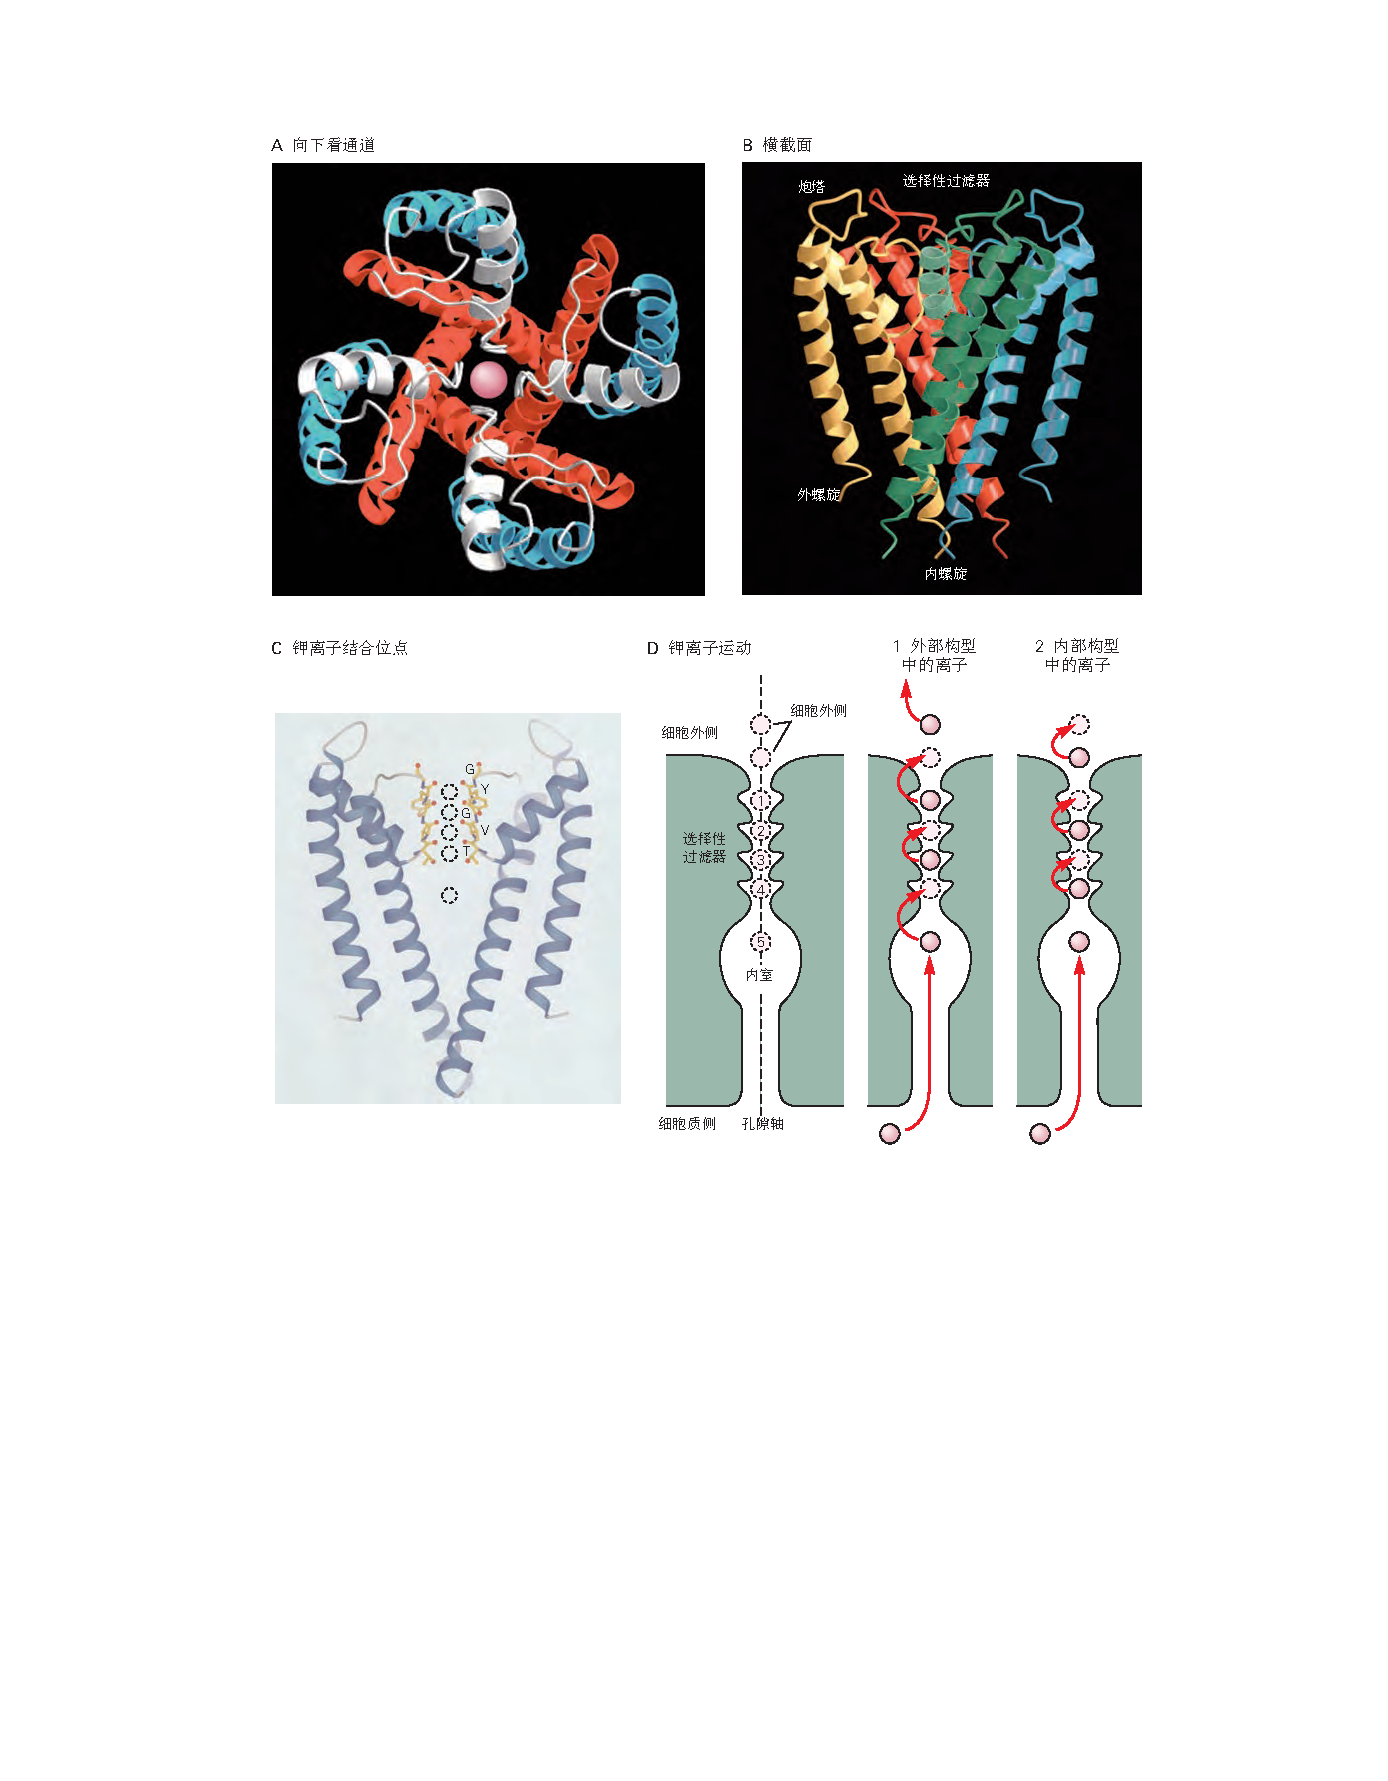
\includegraphics[width=0.9\linewidth]{chap08/fig_8_12}
	\caption{细菌钾通道的 X 射线晶体结构\cite{doyle1998structure}。
		A. 该视图是从细胞外向下看通道孔。
		KcsA \ce{K+} 通道的 4 个亚基中的每一个都贡献两个跨膜螺旋,一个外螺旋(蓝色)和一个内螺旋(红色)。
		P 区(白色)位于通道孔的细胞外表面附近,由一个短的$\alpha$螺旋(孔螺旋)和一个形成通道选择性过滤器的环组成。
		孔的中心是 \ce{K+} 离子(粉红色)。
		B. 在膜横截面内的侧视图中可以看到通道。 4 个亚基以不同的颜色显示。
		C. 与 B 部分相同方向的另一个视图仅显示 4 个亚基中的 2 个。
		该通道包含 5 个 \ce{K+} 结合位点(虚线)。
		其中 4 个位点位于选择性过滤器(黄色)中,而第 5 个位点位于通道中心附近的内腔中。
		选择性过滤器的 4 个 \ce{K+} 结合位点由每个亚基 5 个氨基酸残基的连续氧原子环(红色)形成。
		其中 4 个环由来自 4 个连续氨基酸残基,即甘氨酸(G)、酪氨酸(Y)、甘氨酸(G)和缬氨酸(V)主链主链的羰基氧原子形成。
		选择性过滤器内端附近的第 5 个氧环由苏氨酸(T)的侧链羟基氧形成。
		每个环包含 4 个氧原子,一个来自每个亚基。
		此视图中仅显示了来自 4 个亚基中的两个的氧原子\cite{morais2001energetic}。
		D. \ce{K+} 离子通过通道的渗透视图说明了各种 \ce{K+} 结合位点占用的变化顺序。
		一对离子在选择性过滤器中的一对结合位点之间协同跳跃。
		在初始状态下,即“外部构型”,一对离子结合到位点 1 和 3
		当离子进入通道的内口时,内室中的离子跳跃以占据选择性的最里面的结合位点 过滤器(位点 4)。
		这导致外部结构中的一对离子向外跳跃,从通道中排出一个离子。
		现在处于内部构型(位点 2 和 4)的两个离子可以跳到结合位点 1 和 3,使通道返回到其初始状态(外部构型),从这里它可以传导第二个 \ce{K+} 离子\cite{miller2001see}。}
	\label{fig:8_12}
\end{figure}


来自每个亚基的 4 个内部 $\alpha$-螺旋排列在孔的细胞质末端。
在通道的细胞内口处,这 4 个螺旋交叉,形成一个非常狭窄的开口,即圆锥形帐篷的“烟孔”。
因为这个孔太小而不能让 \ce{K+} 离子通过,因此推测该晶体结构表示通道处于关闭状态。
内部螺旋与电压门控 \ce{K+} 通道的 S6 跨膜片段同源(图 8–11A)。
在通道的细胞外端,每个亚基中的跨膜螺旋由一个区域连接,该区域由 3 个部分组成:
(1)围绕通道口的氨基酸链(炮塔区域),
(2)长度约为 10 个氨基酸的缩写 $\alpha$-螺旋(孔螺旋),向孔的中心轴突出,以及
(3)P 区 C 末端附近的 5 个氨基酸,形成选择性过滤器。


孔隙的形状和结构决定了它的离子传导性能。
孔隙的内口和外口都有酸性氨基酸衬里,其负电荷有助于从溶液中吸引阳离子。
从内到外,孔隙由一条中等宽度的隧道组成,长度为 18 Å,隧道通向一个更宽(直径为 10 Å)的球形内腔。
这个内腔主要由疏水氨基酸侧链构成。
这些相对较宽的区域之后是非常窄的选择性过滤器,长度仅为 12 Å,这是 \ce{K+} 离子通过的速率限制。
如图~\ref{fig:8_12}C、D~所示,从细胞质入口到选择性过滤器的 28 Å 内孔缺乏极性基团,这些极性基团会通过结合和解除结合离子来延缓离子的通过,从而确保了 \ce{K+} 离子的高通过率。


离子从极性溶液通过非极性脂质双分子层时,会遇到双分子层中间能量最低的区域。
\ce{K+} 离子的这两个区域之间的巨大能量差异通过通道结构的两个细节最小化。
如图~\ref{fig:8_12}C~所示,内室充满水,提供高度极性的环境,孔隙螺旋提供偶极子,其电负性羧基末端指向该内室。


20 个电负性氧原子排列在选择性过滤器的壁上,与渗透离子形成有利的静电相互作用,从而部分补偿了 \ce{K+} 离子脱去水合水时产生的高能量成本。
4 个亚基中的每个亚基都有 4 个来自蛋白质骨架的主链羰基氧原子和一个侧链羟基氧原子,总共形成 4 个 \ce{K+} 离子结合位点。
因此,每个结合的 \ce{K+} 离子都能通过与位于结合阳离子上方和下方两个平面中的总共 8 个氧原子的相互作用而稳定。
通过这种方式,该通道能够补偿 \ce{K+} 离子水合水的损失。
如图~\ref{fig:8_12}C~所示,选择性过滤器稳定在一个临界宽度上,这样在 \ce{K+} 离子通过时它就能够提供最佳的静电相互作用,但对于较小的 \ce{Na+} 离子来说太宽了,无法在过滤器长度的任何点与所有 8 个氧原子有效地进行相互作用。


鉴于 \ce{K+} 离子与通道之间的广泛相互作用,KcsA 通道如何管理其高传导率?
尽管该通道总共包含 5 个 \ce{K+} 离子的潜在结合位点,但 X 射线分析表明该通道在任何时刻最多可被 3 个 \ce{K+} 离子占据。
一个离子通常存在于宽阔的内室中,两个离子占据选择性过滤器内 4 个结合位点中的两个(图~\ref{fig:8_12}D)。


这些结构数据导致了以下假设。
由于静电排斥,两个 \ce{K+} 离子永远不会同时占据选择性过滤器内相邻的结合位点;
相反,水分子总是介于 \ce{K+} 离子之间。
在传导过程中,选择性过滤器内的一对 \ce{K+} 离子在成对的结合位点之间串联跳跃。
如果选择性过滤器中只有一个离子,它就会被紧密地结合在一起,离子渗透的吞吐率就会受到影响。
但是占据附近位置的两个 \ce{K+} 离子之间的相互静电排斥确保离子只会短暂停留,从而导致 \ce{K+} 传导的总体速率很高。


KcsA 选择性过滤器的形式似乎在各种类型的哺乳动物电压门控 \ce{K+} 通道中高度保守。
然而,\textit{麦金农}及其同事最近的研究发现,这一典型孔道选择性滤过器下方的几何和表面电荷特征的变化,在如何导致一些电压门控 \ce{K+} 通道在单通道传导性和对各种开放通道阻断剂的亲和力的方面,存在明显差异。


\ce{K+} 通道选择性过滤器和 \ce{K+} 离子之间的紧密配合有助于解释这些通道异常高的选择性,但并不代表所有通道类型。
正如我们将在后面的章节中看到的,在许多通道中,孔径明显大于主要渗透离子,导致选择性较低。



\subsection{电压门控钾通道结构的 X 射线晶体学分析提供了对通道门控机制的深入了解}

如前所述,电压门控离子通道的 S4 段被认为是检测膜电位变化的电压传感器。
S4 中的正电荷如何响应膜电位的变化穿过膜电场?
S4 运动如何与门控耦合?
电压感应区与通道的成孔区有什么关系?
开放通道的配置是什么?
这些问题的一些答案来自哺乳动物电压门控 \ce{K+} 通道的 X 射线晶体学分析,以及使用诱变和其他生物物理学方法的大量研究。
\textit{麦金农}及其同事研究了哺乳动物电压门控 Kv1.2 \ce{K+} 通道,以及密切相关的嵌合体 Kv1.2-Kv2.1,它们产生了更高分辨率的图像。


他们对 Kv1.2 通道和 Kv1.2-2.1 嵌合体的 X 射线晶体结构的分析表明,\ce{K+} 通道亚基具有两个结构域。
S1-S4 区段在通道外围形成电压感应域,而 S5-P-S6 区段在通道中轴形成孔域。
如图~\ref{fig:8_13}~所示,这两个结构域通过短的 S4-S5 偶联螺旋在其细胞内末端相连。
S1-S4 电压传感器是一个独立域的想法得到以下事实的支持:某些细菌蛋白质包含 S1-S4 域但缺少孔域。
一种这样的蛋白质是电压敏感磷酸酶,而另一种形成电压门控质子通道。
相反,如图~\ref{fig:8_11}B~所示,内向整流 \ce{K+} 通道具有高 \ce{K+} 选择性,但由于缺少电压传感器域,因此不直接由电压门控。


\begin{figure}[htbp]
	\centering
	\includegraphics[width=0.9\linewidth]{chap08/fig_8_13}
	\caption{电压门控钾通道的 X 射线晶体结构\cite{long2007atomic}。
		A. 上图:除了其 6 个跨膜 $\alpha$ 螺旋(S1–S6)外,电压门控 \ce{K+} 通道亚基还包含一个短的 $\alpha$-螺旋(P 螺旋)是 P 区选择性过滤器的一部分,以及连接跨膜螺旋 S4 和 S5(4-5 偶联螺旋)的膜细胞质侧的 $\alpha$螺旋。
		底部:单个亚基的 X 射线结构模型显示了 6 个跨膜螺旋、P 螺旋和 4-5 偶联螺旋的位置。
		S1-S4 电压感应区和 S5-P-S6 成孔区位于不同的区域。
		结合在孔中的两个 \ce{K+} 离子以粉红色显示。
		B. 在这个通道的侧视图中,每个亚基都是不同的颜色。
		亚基 6(红色)与 A 部分的方向相同。}
	\label{fig:8_13}
\end{figure}


晶体结构还有助于阐明通道打开时会发生什么。
\textit{克莱$\cdot$阿姆斯特朗}在 1960 年代的研究表明,在高等生物的电压门控 \ce{K+} 通道的细胞内口处存在一个门。
他发现只有当去极化打开这个内门时,\textit{四乙胺}等小有机阳离子才能进入并阻塞通道。
如图~\ref{fig:8_12}~所示,在封闭的细菌 \ce{K+} 通道中,4 个内部跨膜螺旋(对应于电压门控 \ce{K+} 通道中的 S6 螺旋)在其细胞质末端以紧密的束状交叉相交,形成通道的封闭门。
相比之下,Kv1.2–2.1 嵌合体的 S6 螺旋在柔性三氨基酸铰链(脯氨酸-缬氨酸-脯氨酸)处弯曲,导致螺旋的内端向外弯曲。
如图~\ref{fig:8_13}~和图~\ref{fig:8_14}C~所示,这种配置导致开放通道构象,内部孔口直径扩大到 12 Å,宽度足以通过完全水合的 \ce{K+} 离子以及较大的阳离子,如\textit{四乙胺}。
一旦进入通道腔内,\textit{四乙胺}就会阻止 \ce{K+} 渗透,因为它太大,无法通过选择性过滤器。
Kv 通道处于打开状态并不奇怪,因为晶体中的通道上没有电压梯度。
这与将膜去极化至 0 毫伏时的情况类似,在此电压下通道通常处于开放状态。
这种开放机制很可能是一种通用机制,因为细菌和高等生物体内许多 \ce{K+} 通道的内螺旋在这个位置也有一个灵活的铰链。


\begin{figure}[htbp]
	\centering
	\includegraphics[width=0.65\linewidth]{chap08/fig_8_14}
	\caption{基于两个钾通道的 X 射线晶体结构的电压门控模型。
		在图中的每个部分中,左图显示了开放电压门控 Kv1.2-2.1 嵌合体的实际结构,而右图显示了闭合电压门控 \ce{K+} 通道的假设结构,基于 部分关于闭合状态下细菌 \ce{K+} 通道 KcsA 孔区的结构。
		A. 从细胞外俯视开放和封闭通道的视图。
		中央孔在关闭状态下收缩,阻止 \ce{K+} 流过通道。
		B. 从侧面看 S1–S4 电压感应域,平行于膜平面。
		S4 中带正电荷的残基显示为蓝色棒。
		在打开状态下,当膜去极化时,S4 螺旋上的 4 个正电荷位于膜的外半部,面向外部溶液。
		膜内部的正电荷通过与 S1 和 S2(红色棒)中带负电荷的残基相互作用而稳定。
		在关闭状态下,当膜电位为负时,S4 区域向内移动,因此其正电荷现在位于膜的内半部分。
		S4 的向内运动导致细胞质 S4-S5 偶联螺旋(橙色)向下移动。
		C. 电压门控时通道孔的假定构象变化。
		通道的四聚体 S5-P–S6 孔区域的侧视图显示了 S4–S5 耦合螺旋。
		膜复极化导致 S4-S5 螺旋向下运动,向孔的 S6 内螺旋施加力(蓝色)。
		这导致 S6 螺旋在其 pro-val-pro 铰链处弯曲,从而关闭通道的门。}
	\label{fig:8_14}
\end{figure}


一个长期存在的问题涉及 S4 段电压传感器上门控电荷的放置和移动。
如前所述,这些电荷随着膜电位的变化而在膜平面内移动,这被认为是膜去极化与通道门控的耦合。
然而,在疏水膜内放置电荷会导致不利的能量状态,正如前面讨论的溶液中的游离离子一样。
离子通道如何补偿这种不利的自由能?


晶体结构为这个问题提供了一些答案。
诱变研究表明,S4 区段外半部的 4 个带正电荷的精氨酸残基可能携带大部分门控电荷。
在开放状态下,4 个正电荷向外朝向膜的细胞外侧,在那里它们可能与水或磷脂双层的带负电荷的头基发生能量上有利的相互作用。
通过与 S1-S3 跨膜螺旋上带负电荷的酸性残基的相互作用,位于脂质双层内更深处的其他 S4 残基上的正电荷得以稳定。


目前,还没有 Kv1.2-Kv2.1 嵌合体封闭状态的晶体结构。
然而,如图~\ref{fig:8_14}~所示,\textit{麦金农}及其同事提出了一种基于开放电压门控 \ce{K+} 通道和闭合细菌 \ce{K+} 通道 KcsA 结构的合理电压门控模型。
根据该模型,细胞内的负电压对带正电的 S4 螺旋施加力,使其向内移动约 1.0 至 1.5 纳米。
因此,4 个带正电荷的 S4 残基,在去极化状态下面向外部环境并感知细胞外电位,现在则面向膜的细胞内侧并感知细胞内电位。
这样,当通道在关闭态和打开态之间转换时,每个 S4 区段的移动将在膜电场中转移 3 到 4 个门控电荷,每个四聚体通道总共移动 12 到 16 个电荷。 
这个数字与生物物理测量得出的门控电荷移动总量相似(第~\ref{chap:chap10}~章)。


S4 运动与通道栅极是如何耦合的?
根据该模型,当膜电压变为负值时,S4 段向内运动,从而对 S4-S5 耦合螺旋产生向下的力。
该螺旋在其细胞质表面大致平行于膜,在打开状态下位于 S6 螺旋门的内端。
当 S4-S5 螺旋向下移动时,它充当杠杆,向 S6 施加力并关闭门。
因此,人们认为电压传导依赖于通道的电压传感域和孔隙域之间的机电耦合。
尽管这种机电耦合模型为膜电压变化如何导致通道门控提供了令人满意的描述,但要明确回答这一关键问题,还需要解析相关电压门控哺乳动物 \ce{K+} 通道的闭合状态结构。


大多数电压门控 \ce{K+} 通道以及电压门控 \ce{Na+} 和 \ce{Ca+} 通道都存在通道传感元件(S4/S4-S5 连接器)与孔门(S6)之间的这种直接耦合。
然而,在许多情况下,通道中直接响应门控信号的元件并不与通道门直接接触,而是由一种变构机制通过更远的构象变化间接传播响应。
例如,在电压门控 \ce{K+} 通道 Kv10 中,S4-S5 连接器无法充当 S6 上的杠杆。
相反,S4 响应负电势而向内移动,通过横向压缩紧贴 S6 螺旋的 S5 螺旋间接关闭 S6 门。
稍后将在电压门控 \ce{Na+} 通道失活(第~\ref{chap:chap10}~章)和配体门控(第~\ref{chap:chap12}~和~\ref{chap:chap13}~ 章)和机械门控通道(第~\ref{chap:chap18}~章)激活的背景下讨论变构门控机制的其他情况。



\subsection{\ce{Cl-} 通道选择性渗透的结构基础揭示了通道和转运蛋白之间的密切关系}

离子通过离子转运蛋白或泵的主动转运以及通过离子通道的被动扩散穿过细胞膜。
离子转运蛋白与离子通道不同,因为
(1)它们利用能量源,逆着电化学梯度主动转运离子,并且
(2)它们以远低于离子通道的速率传输离子,该速率太低而无法支持快速神经元信号传导。
然而,根据对 CLC 蛋白质家族的研究,某些类型的转运蛋白和某些离子通道具有相似的结构。


在脊椎动物中表达的 CLC 蛋白由一个 \ce{Cl-} 通道家族和一个密切相关的 \ce{Cl-}-\ce{H+} 协同转运蛋白家族组成。
协同转运蛋白利用一个离子的电化学梯度使另一个离子逆着其电化学梯度移动。
在细胞内细胞器中表达的 CLC \ce{Cl-}\ce{H+} 协同转运蛋白将两个 \ce{Cl-} 离子跨膜转移以换取一个质子。
这种类型的转运蛋白称为离子交换剂。


人体电压门控 ClC-1 通道对于维持骨骼肌的静息电位很重要(第~\ref{chap:chap57}~章)。


\textit{麦金农}及其同事已确定人类 ClC-1 通道和同源大肠杆菌 CLC 交换器的晶体结构。
他们发现,氨基酸序列的相似性反映在整体结构的明显相似性上。
这两种 CLC 蛋白都是由两个相同的亚基组成的同型二聚体。
如图~\ref{fig:8_15}~所示,每个亚基形成一个单独的离子通路,两个亚基独立发挥作用。
CLC 蛋白的结构与 \ce{K+} 通道的结构完全不同。
与中心区域最宽的 \ce{K+} 通道的孔不同,CLC 蛋白的每个孔都具有沙漏轮廓。
沙漏的颈部是一条 12 Å 长的隧道,它构成了选择性过滤器,其宽度刚好足以包含 3 个完全脱水的 \ce{Cl-} 离子。


\begin{figure}[htbp]
	\centering
	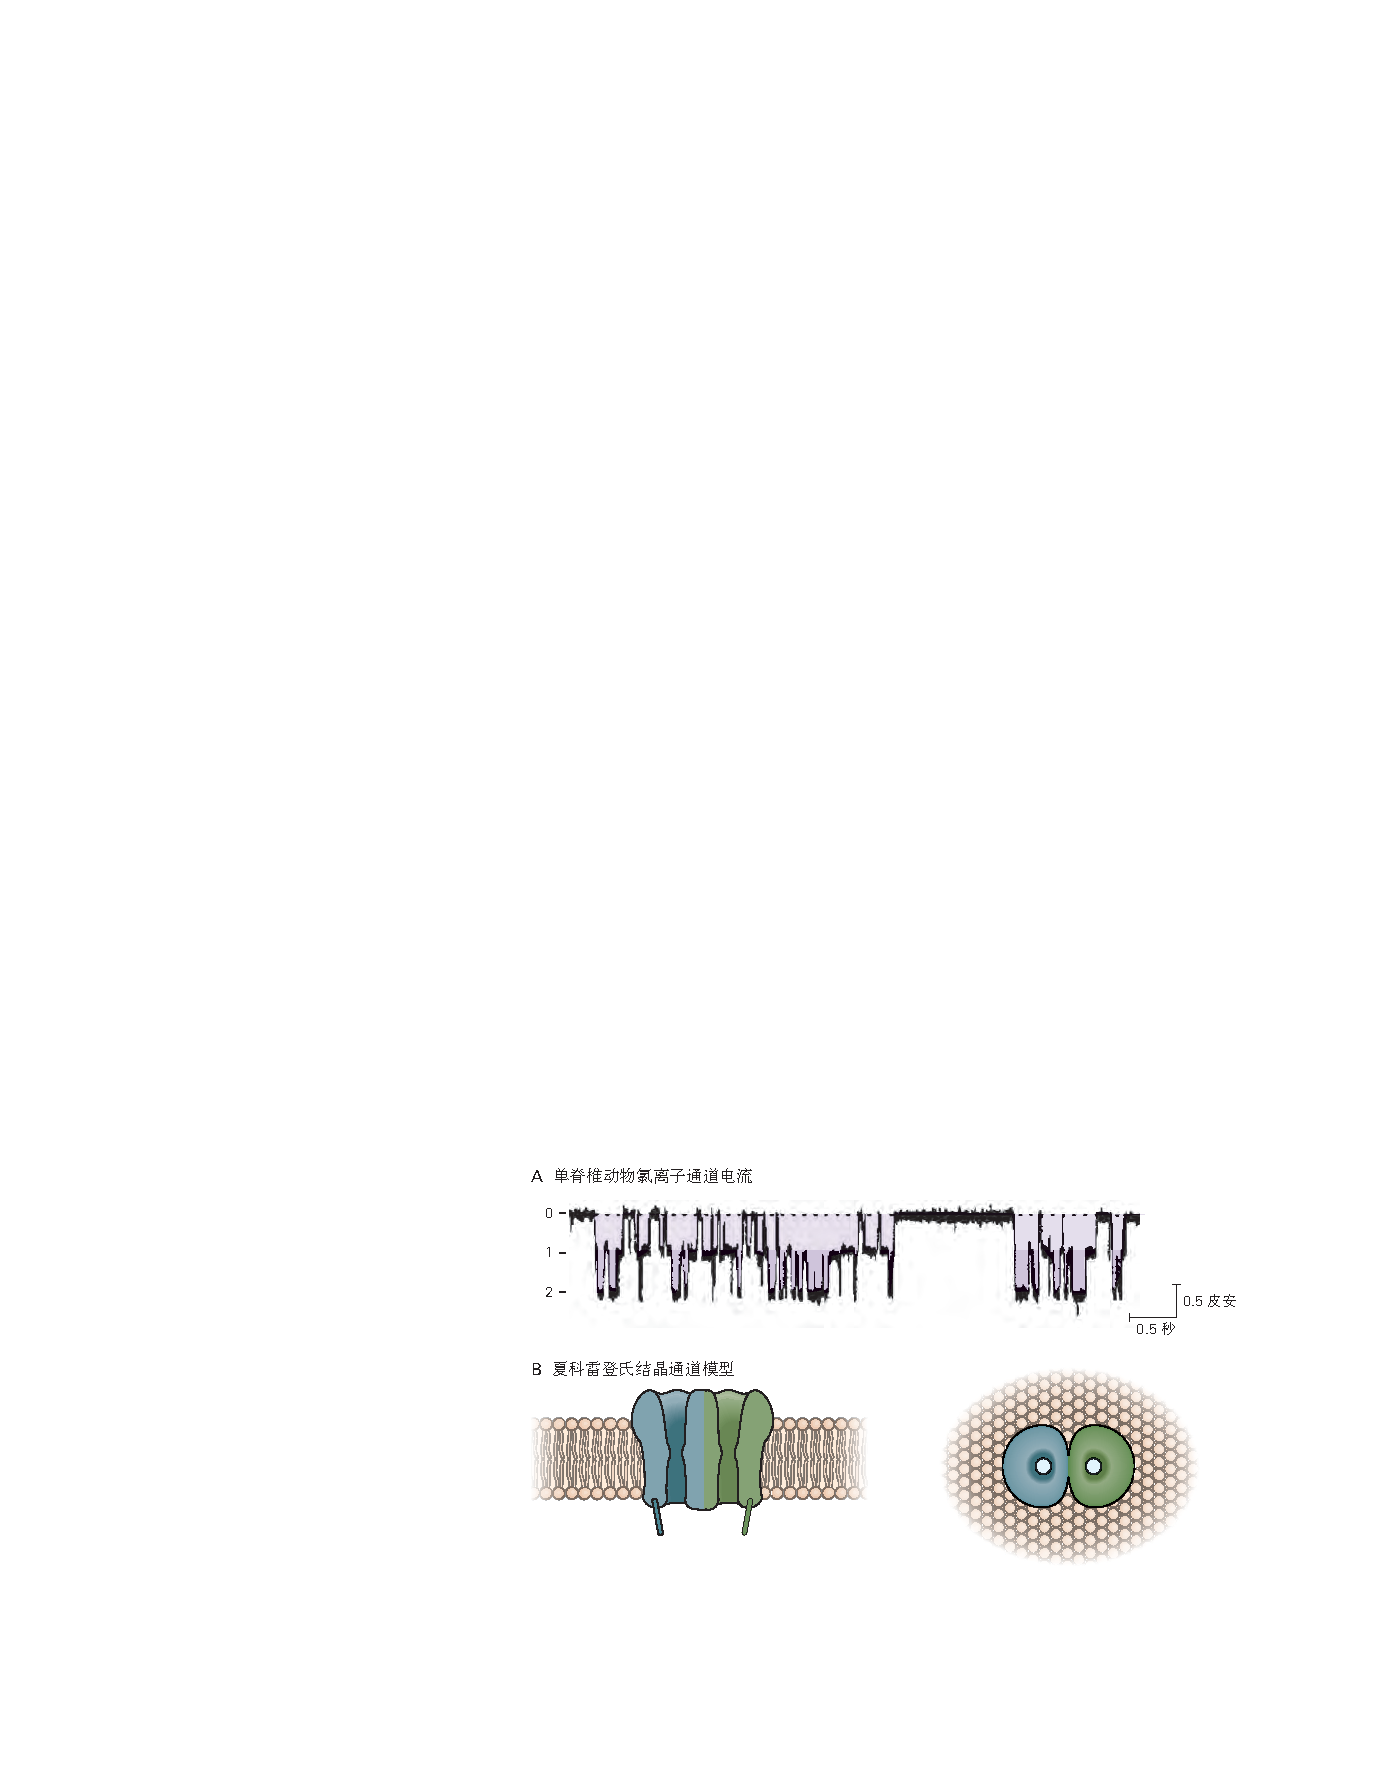
\includegraphics[width=0.8\linewidth]{chap08/fig_8_15}
	\caption{\ce{Cl-} 通道和转运蛋白的脊椎动物 CLC 家族是具有两个相同孔的双桶通道。
		A. 通过单个脊椎动物 \ce{Cl-} 通道的电流记录显示 3 个级别的电流:两个孔都关闭(0),一个孔打开(1),两个孔都打开(2)。
		B. 从侧面(左)显示通道并从细胞外向下看膜(右)。
		每个亚基都包含自己的离子传输通路和门。
		此外,二聚体有一个由两个亚基共享的门(未显示)。}
	\label{fig:8_15}
\end{figure}


尽管 CLC 蛋白和 \ce{K+} 通道的离子渗透途径在显著方面不同,但它们已经进化出 4 个对其功能至关重要的相似特征。
首先,它们的选择性过滤器包含渗透离子的多个顺序结合位点。
多离子占据形成了一种可促进离子快速通过的可变状态。
其次,离子结合位点是由极性的、部分带电的原子形成的,而不是由完全电离的原子形成的。
由此产生的相对较弱的结合能确保渗透离子不会过于紧密地结合在一起。
第三,渗透离子通过两个 $\alpha$-螺旋的正极化末端稳定在膜的中心。
第四,选择性过滤器两端的宽阔充水前庭允许离子以部分水合状态接近过滤器。
因此,尽管 \ce{K+} 通道和 CLC 蛋白在氨基酸序列和整体结构上存在根本差异,但在这两类膜蛋白中进化出惊人相似的功能特征,促进了高度的离子选择性和高效的通量。 
从原核生物到人类,这些特征都以惊人的保真度保存下来。


需要进行更详细的结构研究,才能了解一些 CLC 蛋白如何发挥 \ce{Cl-}\ce{H+} 交换器的功能,而另一些则发挥传统通道的作用。
大多数交换器和泵,例如\textit{钠钾泵}(第~\ref{chap:chap9}~章),被认为有两个门,一个在外部,一个在内部,它们永远不会同时打开。
相反,如图~\ref{fig:8_16}~所示,离子运动和门运动被认为是紧密耦合的反应循环的一部分。
CLC 交换器显然有两个控制 \ce{Cl-} 通量的门,与选择性过滤器中柔性谷氨酸残基的质子化-去质子化循环耦合,使质子穿过膜。
由此产生的构象变化使 \ce{Cl-} 能够逆其浓度梯度传输,这是由 \ce{H+} 离子沿其电化学梯度向下流动驱动的。
CLC 通道的结构显然与转运体十分相似,只是在离子转运途径中具有改进的门和微小的结构变化,从而使 \ce{Cl-} 沿着其电化学梯度更快速地移动。


\begin{figure}[htbp]
	\centering
	\includegraphics[width=1.0\linewidth]{chap08/fig_8_16}
	\caption{离子通道与转运蛋白或泵之间的功能差异\cite{gadsby2004spot}。 
		A. 离子通道具有连续的水通道,用于跨膜离子传导。
		关闭门可以关闭此路径。
		B. 离子泵和传输器有两个串联的门控制离子通量。
		门永远不会同时打开,但两者都可以关闭以将一种或多种离子捕获在孔中。
		此处所示的转运蛋白类型使两种不同类型的离子沿相反方向移动,称为交换器或逆向转运蛋白。
		离子运动与两个门的打开和关闭循环紧密相关。
		当外部门打开时,一种离子离开,而另一种离子进入孔(1)。
		这会触发构象变化,导致外部门关闭,从而捕获进入的离子(2)。
		然后,第二次构象变化导致内门打开,允许被捕获的离子离开并允许新离子进入(3)。
		进一步的构象变化关闭内部门,允许循环继续(4)。
		在每个循环中,一种类型的离子从细胞外部传输到细胞内部,而另一种类型的离子从细胞内部传输到细胞外部。
		通过耦合两个或多个离子的运动,交换器可以使用存储在一个离子的电化学梯度中的能量来主动地逆着其电化学梯度传输另一个离子。}
	\label{fig:8_16}
\end{figure}



\section{亮点}


1. 离子通过两大类完整的膜蛋白:离子通道和离子泵或转运蛋白,来穿过细胞膜。


2. 离子通道是离子被动跨膜流动的催化剂。
 离子通道的中央有一个充满水的孔隙,以代替膜两侧的极性环境。
它允许带电离子在离子的电化学梯度的驱动下快速穿过细胞膜的非极性环境。


3. 大多数离子通道对某些离子具有选择性渗透性。
通道孔的一部分称为选择性过滤器,根据离子的电荷、大小以及与排列在孔壁上的氨基酸的物理化学相互作用,确定哪些离子可以穿透。


4. 离子通道的闸门可根据不同的信号打开或关闭。
在开放状态下,通道产生离子电流,产生快速电压信号,在神经系统和其他可兴奋细胞中携带信息。


5. 大多数离子通道具有 3 种状态:开放、关闭和失活或脱敏。
这些状态之间的转换称为门控。
根据通道的类型,门控受多种因素控制,包括膜电压、配体结合、机械力、磷酸化状态和温度。


6. 神经和肌肉细胞中最常见的离子通道属于三大基因超家族,其成员通过基因序列同源性相关,并且在大多数情况下通过功能特性相关。


7. 大多数离子通道由多个亚基组成。
这些亚基的组合排列可以产生具有不同功能特性的多种通道。 转录后修饰产生更多的多样性。


8. 各种类型的离子通道在不同类型的神经元和神经元的不同区域有不同的表达方式,从而提高了神经系统的功能复杂性和计算能力。
一些离子通道和转运蛋白的表达模式在发育过程中会发生变化,并随着神经元活动模式的变化而变化。


9. 不同类型神经元中的离子通道种类繁多,促使人们集中精力开发能够激活或阻断神经和肌肉细胞中特定通道类型的药物。
这类药物原则上可以最大限度地提高疗效,同时将副作用降到最低。


10. 电压门控离子通道的结构功能和 X 射线晶体学研究为 \ce{K+} 通道传导、选择性和门控的分子和原子级细节提供了重要见解。
单粒子冷冻电子显微镜的最新技术进步导致对各种离子通道的研究取得了快速进展。


11. 主动转运由称为转运体或泵的整体膜蛋白介导,使离子能够逆着电化学梯度穿过膜。
产生主动离子通量的驱动力,要么来自化学能(\textit{三磷酸腺苷酶}的水解),要么来自共转运离子的有利电化学势差。


12. 大多数离子传输器和泵并不为离子提供连续通道。
相反,它们在运输周期的不同阶段会发生构象变化,从而使分子的中心腔交替进入膜的两侧。
由于这些构象变化相对缓慢,因此它们在介导离子通量方面的效率远远低于离子通道。



